\documentclass[twoside, a4paper]{article}
\usepackage[inner=2cm, outer=2cm, top=2cm, bottom=2cm, includeheadfoot]{geometry} 


\usepackage[most]{tcolorbox}
% \usepackage{amsmath}
\usepackage{amssymb}
\usepackage{shortcut}
\usepackage{graphicx}
% \usepackage{subfig}

% \usepackage{import}
% \usepackage[Sonny]{fncychap}
% \usepackage{fancybox}
% \usepackage{dsfont}
% %\usepackage{appendix}
% \usepackage{lipsum}
% \usepackage[toc,page]{appendix}
% \usepackage{hyperref}
% \newcommand{\RomanNumeralCaps}[1]
%     {\MakeUppercase{\romannumeral #1}}
% \usepackage[toc,page]{appendix}
% \usepackage{tabularx}
% \setlength{\parindent}{0cm}

\renewcommand{\familydefault}{\sfdefault }

% \usepackage{titlesec}

% \setcounter{secnumdepth}{4}

% \titleformat{\paragraph}
% {\normalfont\normalsize\bfseries}{\theparagraph}{1em}{}
% \titlespacing*{\paragraph}
% {0pt}{3.25ex plus 1ex minus .2ex}{1.5ex plus .2ex}

% \usepackage{stackengine}



% % \(\stackunder{D}{\text{..}}\)em\(\stackon{a}{\text{\small $\cup$}}\)ntu
\title{ Njang/jàng Xayma}
\author{SARR Georges Mbissane}
\date{Ci wéeru ñaari junni ak ñaar fukk ak ñaar (2022)}


\begin{document}

\maketitle


% \section{\(\stackunder{H}{\text{..}}\)araf}
% \section{Dugalinu mbir (Introduction)}
% % \(\stackunder{T}{\text{..}}\)i bir t\(\stackon{e}{\text{..}}\)ré bilé, damay \(\stackunder{d}{\text{..}}\)éma téki (lapato) lu baréwul (lu tûti) ci bir \(\stackunder{h}{\text{..}}\)am\(\stackunder{h}{\text{..}}\)amu Mathématiques.\\

% Ci bir téeré bilé, damay jéema jangalé Xayma. Sama ñàkk déeg Wolof, mba njumté, mën nañ ma téré bind lou joub (wër). Kena ku gis la ko nourou njumté, mën na ma yoné bataaxal fi: georgesmbissanes@gmail.com. \\

% Ay baat you am solo:
% \begin{itemize}
%     \item jéemantu: exercice ?
%     \item njumté: erreur
%     \item lim: compter/nombre
%     \item mandargal: représenter ? -> royukaay ? (exemple) 30 moy mandargal fanweer
%     \item nguir leeraal: pour expliquer
%     \item saam: ensemble ?
%     \item këraleg: tableau ?
%     \item tontu: réponse
%     \item nafar: souvenir ? en lien avec nafa -> Bourse, Poche, Porte-feuille (objet qui permet de garder un autre objet)
%     \item tegtal ? : indication ?
%     \item nataal: image
%     \item njem: entreprise dans le sens d'entreprendre ?
%     \item jumtukaay: outil
%     \item xaymakaay/jumtukaay xayma: calculatrice
%     \item cax: devinette/problème ? exemple: (caxu Xayma) problème en mathématiques
%     \item ac/toxal: retenue (dans les opérations arithmétiques)
%     \item tomb: point
%     \item ëmbef: élément ?
%     \item mboolo: group
%     \item $a$ ñu toftal ci $b$: on met $b$ après $a$ ? 
%     \\
% \end{itemize}

% Top leen lëkaalekaay yilé ngir gis luma jappalé ba ma bind Xayma ci Wolof, ñoom ñoy saama sukëndikukaay:
% \begin{itemize}
%     \item \href{https://www.youtube.com/@ecolesausenegal/search?query=cours%20mathematiques%20wolof}{Youtube: Ecoles au Senegal, Cours - Mathématiques - Wolof *}
%     \item \href{https://fr.glosbe.com/}{https://fr.glosbe.com/}
%     \item \href{https://ia801303.us.archive.org/29/items/dictionnairesfra00holy/dictionnairesfra00holy.pdf}{Dictionnaire Wolof-Français, Français-Wolof} (baatukay bu magét la nak)
% \end{itemize}

% \section{Mbind Xayma (Notations en Mathématiques)}
% Mbid\footnote{notation ?} Xayma lu am solo la, ndaxte da nuy yombalal deeg-deeg ak leeral rëd Xayma.

% \subsection{Sëfu Xayma (Opérations)}
%     Amal $(a,b) \in E$ (manam amal $a$ ak $b$, ñaari ëmbefu\footnote{élément ?} been ëmbe\footnote{ensemble ?} $E$).
% \begin{itemize}
%     \item $a$ ñu yokk/doli(?) ci $b$ muy $c$: $a + b = c$ 
%     \item $a$ ñu wañi ci $b$ muy $c$: $a - b = c$ 
%     \item $a$ ñu ful ko ak $b$ muy $c$: $a \times b = c$ 
%     \item $a$ ñu seddale ko ak $b$ muy $c$: $a / b = c$ 
%     \item \textbf{Seetlu (Remarque)} 
%         \begin{itemize}
%             \item[$\bullet$] Nañu bayi hel ke ni $a + b = b + a$, $a \times b = b \times a$
%         \end{itemize}
% \end{itemize}

% \subsection{Lim}
% \subsubsection{Limu been been yi (bb) (unités de 0 à 9) ak limu fukk fukk yi (ff) (dizaines de 10 à 99)}
%     \begin{itemize}
%         \item tus (0), been (1), ñaar (2), ñatt (3), ñeent (4), juròom (5), juròom-been (6), juròom-ñaar (7), juròom-ñatt (8), juròom-ñeent (9), fukk (10), fukk ak been (11), ..., fukk ak juròom-ñeent (19),
%          \item ñaar-fukk (20), ñaar-fukk ak been (21), .., ñaar-fukk ak juròom-ñeent (29)
%          \item fanweer (30), fanweer ak been (31), ..., fanweer ak juròom-ñeent (39)
%          \item ñeent-fukk (20), ñeent-fukk ak been (21), .., ñeent-fukk ak juròom-ñeent (49)
%          \item ...
%          \item juròom-ñeent-fukk (90), juròom-ñeent-fukk ak been (91), .., juròom-ñeent-fukk ak juròom-ñeent (99)
%          \item fukk fukk (ff) (dizaine), been been (bb) (unité) 
%     \end{itemize}
% \subsubsection{Limu téeméer téeméer yi (tt) (centaines) ak limu junni junni yi (jj) (milliers)}
%      \begin{itemize}
%          \item téeméer (100), téeméer ak been (101), téeméer ak .. (yok filé limu been been yi, wala limu fukk fukk yi), téeméer ak juròom-ñeent-fukk ak juròom-ñeent (199)
%          \item ñaar téeméer (200), ñaar téeméer ak been (201), .., ñaar téeméer ak juròom-ñeent-fukk ak juròom-ñeent (299)
%          \item ...
%          \item juròom-ñeent téeméer (900), juròom-ñeent téeméer ak been (901), .., juròom-ñeent téeméer ak juròom-ñeent-fukk ak juròom-ñeent (999)
%          \item Junni (1.000), juròom-been-junni (6.000), fukk-junni (10.000), fukk-junni ak juròom-ñatt ak ñaar-fukk ak ñatt (18023), fanweer-junni ak juròom ak ñeent-téeméer ak been (35401), juròom-ñaar-fukk-junni ak juròom-been ak ñeent-téeméer ak ñaar-fukk ak ñatt (76423).
%      \end{itemize}





 

% \section{Wallum tuutal ak yaatal (Optimisation)}
% \footnote{Manam jëlël been doxalin bi jël ab ëmbefu $\R^n$ juraal ko ab ëmbefu $\R$, wala itam been doxalin bi yob been ëmbefu $\R^n$ ci been ëmbefu $\R$}Amal ab doxalin\footnote{fonction ?} $f: \R^n \longrightarrow \R$ . Amal itam been ëmbef $\Omega$ bu nek ci $\R^n$, ñu kay bindé $\Omega \subset \R^n$. Tuutal $f$ ci biir $\Omega$, mo di seet ci biir $\Omega$, yan ëmbef $x$ (ksë) ño gënë tuutilé $f(x)$ (fe wu ksë) ci ëmbef yëp yu nekk ci biir $\Omega$. Yaatal $f$ ci biir $\Omega$, mo di seet ci biir $\Omega$, yan ëmbef $x$  ño gënë rëylé $f(x)$ ci ëmbef yëp yu nekk ci biir $\Omega$.


\section{Ëmb}
\begin{tcolorbox}[enhanced jigsaw,breakable,pad at break*=1mm,
    colback=red!5!white,colframe=white!75!black,title= Téeki,
    watermark color=white]
  Nañu wowee ëmb, beep saamu cër\footnote{élément} yu ñuy wowee ëmbeef. Amal been ëmb $E$, da ñuy né $x$ ëmbeefu $E$ la, ta ñu ko bindé $x\in E$\footnote{Mën na ñu ko liré "$x$ mu ngi ci biir $E$"}, bu féké ni $x$ ci biir $E$ la nek/la bok.
\end{tcolorbox}

\begin{itemize}
    \item $\N, \Z, \Q, \R$ ay ëmb la ñu.
    \item $\{a, b, c, d, ... z\}$ moy ëmb bu am ab ëmbeef $a$, $b$, $c$, ..., ba $z$
    \item $\emptyset$ moy mbindu ëmb bu amul tus, manam ëmb bu amul been ëmbeef.
    \item $\{a, b\} = \{b, a\}$
\end{itemize}

\begin{figure}[h]
    \centering
    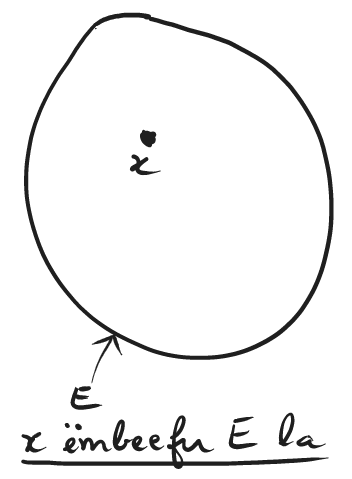
\includegraphics[scale = 0.5]{image/embeefu_emb.png}
    % \caption{}
    \label{fig:my_label}
\end{figure}


\end{document}